\documentclass[conference]{IEEEtran}

\usepackage{amsmath,amssymb,amsfonts}
\usepackage{algorithmic}
\usepackage{subcaption}
\usepackage{graphicx}
\usepackage{textcomp}
\usepackage{xcolor}
\usepackage{svg}
\usepackage[style=ieee]{biblatex}

\addbibresource{references.bib}

\def\ns3{ns-3}

\begin{document}

\title{Extending Energy Models for Wireless Network Simulation with FMI-based Hybrid Co-Simulation}

\author{\IEEEauthorblockN{Lars Moons}
\IEEEauthorblockA{\textit{Department of Computer Science} \\
\textit{University of Antwerp}\\
lars.moons@student.uantwerpen.be}
}

\maketitle

\begin{abstract}
TODO
\end{abstract}

\begin{IEEEkeywords}
energy modeling, co-simulation, wireless network simulation, \ns3, FMI
\end{IEEEkeywords}

\section{Problem Statement}

Energy modeling is a critical aspect of evaluating the performance of wireless network protocols.
Therefore, in the network simulator \ns3, a generic energy model \cite{wu2012energy}
is provided, with basic structures for modeling energy sources.
While there are some pre-built classes available, more advanced energy models require programmers to write their own code.
In a previous study \cite{capuzzo2021ns}, the authors encountered this situation, when they modeled a battery-less IoT device with energy harvesting using the \ns3 energy model interface.
Their workflow involved creating a circuit diagram, solving the circuit using analysis techniques, and implementing the resulting formula in code. 
This approach proves effective for smaller and less complex circuits.
However, when more realism is necessary, this workflow becomes challenging due to potential errors, time consumption, and unfamiliarity with circuit analysis techniques. Furthermore, integrating energy models developed by different teams using different toolsets can pose difficulties.

To overcome these limitations, we propose a new workflow that incorporates visual design, drag-and-drop functionality, and predefined model building blocks \cite{carreira2020foundations}. Existing tools like OpenModelica and Simscape offer such functionality, but they do not directly integrate with discrete-event simulators like \ns3. Hence, the challenge lies in combining these two environments through hybrid co-simulation.
The integration can be made possible with the Functional Mock-up Interface (FMI) standard, which enables communication between the two environments.
Previous work in \cite{cremona2019hybrid}, \cite{cremona2016step}, and \cite{tavella2016toward} has explored FMI-based hybrid co-simulation, but its application to simulating energy models in wireless network simulations appears to be a novel contribution.

In the following sections, we will review discrete-event and physical simulation, discuss the FMI standard, and present the implementation using two APIs: one based on Python and another based on C++. We will also address the challenges encountered during the implementation process and provide guidelines for future work.

\section{Discrete-Event Simulation}

A discrete-event simulator models systems where events occur at specific points in time.
Each event marks a change of state in the system, and states can only change when events take place. 
The simulator maintains a queue of events that are scheduled to execute at a specified simulation time.
These events are executed in sequential time order.
After an event is completed, the simulator proceeds to the next event in the queue or terminates if there are no more events remaining.
Discrete-event simulators are often used in network simulators to model events such as
packet transmission or changes in network topology \cite{riley2010ns}.
Two popular open-source frameworks in this domain are \ns3 and OMNeT++.

\begin{figure}[htbp]
  \centering
  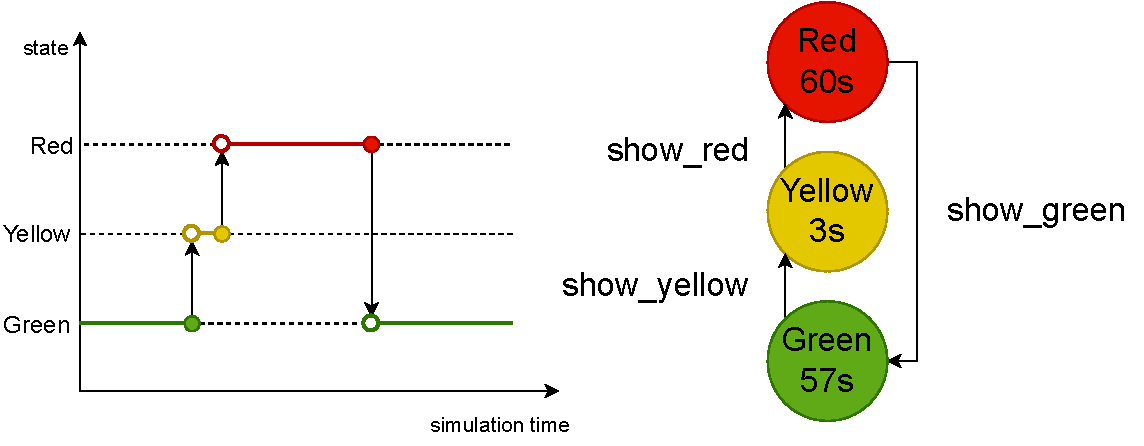
\includegraphics[width=\linewidth]{images/traffic-light.drawio.pdf}
  \caption{Discrete-event system of a traffic light.}
  \label{traffic-light}
\end{figure}

A simple example of a discrete-event system is a traffic light, see Fig. \ref{traffic-light}.
The traffic light has three states: \texttt{RED}, \texttt{YELLOW} and \texttt{GREEN},
and is controlled by three events: \texttt{show\_red}, \texttt{show\_yellow} and \texttt{show\_green}, which set the traffic light to the colour indicated by their names.
The system starts in the \texttt{GREEN} state and schedules the \texttt{show\_yellow} event to occur after 57 seconds.
The simulator advances the simulation time to 57 seconds and executes the \texttt{show\_yellow} event.
During this event, the traffic light transitions to the \texttt{YELLOW} state, and the \texttt{show\_red} event is scheduled to execute after 3 seconds, relative to the current simulation time.
Continuing the simulation, the time is advanced to 60 seconds and the \texttt{show\_red} event is executed.
As a result, the traffic light transitions to the \texttt{RED} state, and the \texttt{show\_green} event is scheduled to execute after 60 seconds.
After that, the simulation time is advanced to 120 seconds, and the \texttt{show\_green} event is executed.
This returns us to the initial state, and the process repeats.

\section{Physical Simulation}

Physical simulation utilises mathematical equations to model the behaviour of physical objects.
Unlike the discrete events, it operates in a continuous state space.
Two popular tools that support physical simulation are OpenModelica and Simscape.
These tools are available either as open-source software or free for academic research.
They eliminate the need to numerically solve systems of equations that govern the laws of physics.
Instead, they provide pre-written blocks that can be connected graphically and let the solver do all the tedious work.
In addition to their graphical interfaces, these tools also support their own modeling language. These languages resemble regular programming languages but operate at a higher level of abstraction.
They are equation-based rather than assignment-based, enabling acausal data flow that does not fix input or output variables.
This flexibility allows inputs and outputs to be derived depending on the situation.
These concepts will be made more clear with an example.

Let's consider a simple physical system, such as a discharging capacitor, see Fig. \ref{capacitor-discharge}.
The system consists of two main components: a capacitor and a resistor.
Using the aforementioned tools, these components can be connected graphically see Fig. \ref{cd:graphical-model}.
The graphical model is then translated into a textual modeling language, see Fig. \ref{cd:modeling-language}.
In this language, the behaviour of a discharging capacitor is described in a differential equation:
\[
\frac{dV}{dt} = -\frac{V}{CR}
\]
Afterwards, in Fig. \ref{cd:numerical-solution}, the equation is solved numerically using Euler's method which approximates the derivative by finite differences:
\[
y'(t_0) \approx \frac{y(t_0+h) - y(t_0)}{h}
\]
Note that this example does not necessarily illustrate the exact working of OpenModelica or Simscape, but it aims to provide intuition.

\begin{figure}[htbp]
  \centering
  \begin{subfigure}[b]{\linewidth}
    \centering
    \includesvg[width=0.4\linewidth]{images/capacitor-discharge-graphical.svg}
    \caption{Graphical model}
    \label{cd:graphical-model}
  \end{subfigure}
  
  \vspace{1em}
  
  \begin{subfigure}[b]{\linewidth}
    \centering
    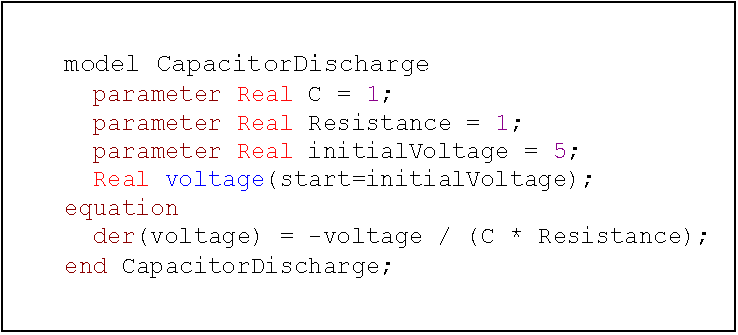
\includegraphics[width=0.9\linewidth]{images/capacitor-discharge-code.drawio.pdf}
    \caption{Modeling language}
    \label{cd:modeling-language}
  \end{subfigure}
  
  \vspace{1em}
  
  \begin{subfigure}[b]{\linewidth}
    \centering
    \includesvg[width=0.9\linewidth]{images/capacitor-discharge-plot.svg}
    \caption{Numerical solution}
    \label{cd:numerical-solution}
  \end{subfigure}
  
  \caption{Physical system of a discharging capacitor.}
  \label{capacitor-discharge}
\end{figure}

\section{FMI standard}

TODO

\section{Python Implementation}

TODO

\section{C++ Implementation}

TODO


\printbibliography

\end{document}
